% Generated by tools/generate_statements_only_paper.py.
% Do not edit this derived file; edit the canonical paper source instead.

\section{Detailed Area-Loss Estimates}
\label{sec:area}

This section records the local inequalities and cyclic estimates used in the
area-loss argument.

Let
\[
 A_\triangle=\frac{\sqrt3}{4}
\]
be the area of a unit equilateral triangle.  Throughout this section areas
are divided by $A_\triangle$.  Thus a unit triangle has normalized area one
and $H$ has normalized area six.

\begin{figure}[H]
\centering
\begin{minipage}[b]{.48\textwidth}
\centering
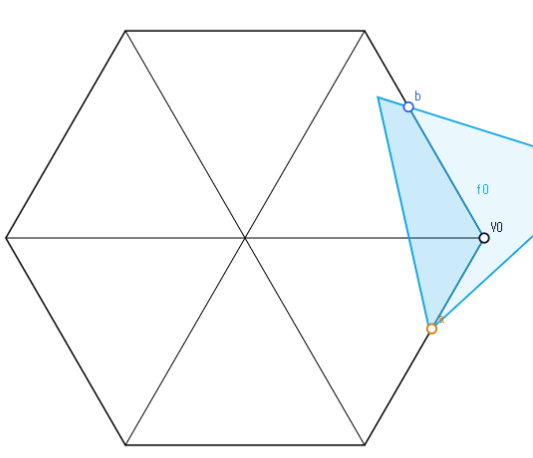
\includegraphics[width=\linewidth]
  {figures/strategy3_local_area_loss.png}
\par\smallskip
\footnotesize (a) local retained area
\end{minipage}\hfill
\begin{minipage}[b]{.48\textwidth}
\centering
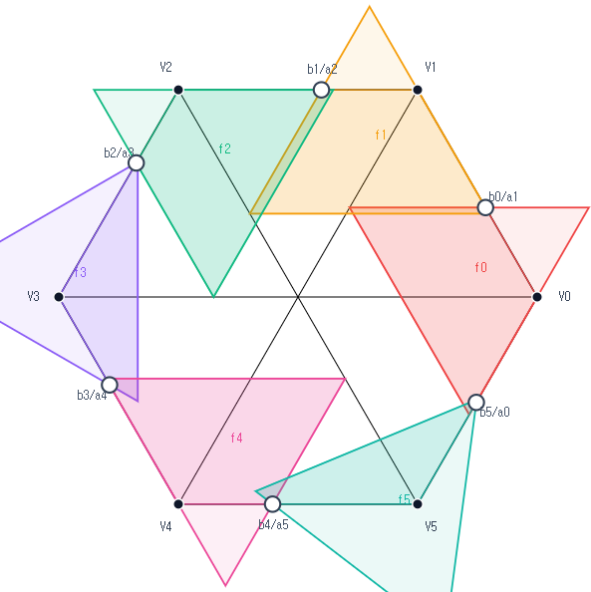
\includegraphics[width=\linewidth]
  {figures/strategy3_global_area_loss.png}
\par\smallskip
\footnotesize (b) global retained areas
\end{minipage}
\caption{Schematic views of Method~3, not to scale.  The local panel
shows one V triangle with boundary reaches $a,b$, and the global panel
shows the six cyclic triangles.  Only the darker portions represent area
retained inside $H$; the stated inequalities, rather than the picture, give
the comparison.}
\label{fig:area-loss}
\end{figure}

\subsection{The local square-loss inequalities}

Fix a vertex $V_i$.  Let $P_a$ and $P_b$ be the points at distances $a$ and
$b$ from $V_i$ on its incoming and forward boundary edges.  For a closed
unit equilateral triangle $T$ containing $V_i,P_a,P_b$, put
\[
 \mathcal L(T)=\frac{\operatorname{area}(T\setminus H)}{A_\triangle}.
\]
Equivalently, if
\[
 f(a,b)=\max_T\frac{\operatorname{area}(T\cap H)}{A_\triangle},
 \qquad \mathcal L(a,b)=1-f(a,b),
\]
then $\mathcal L(a,b)$ is the least possible normalized loss.  Reflection in the
radial axis interchanges $a$ and $b$, and increasing either reach lower bound can only
decrease $f$.

\begin{lemma}[Local wedge reduction]
\label{lem:area-wedge}
After rotating indices to $i=0$, write
\[
 X=V_0+x(V_1-V_0)+y(V_5-V_0),
 \qquad W=\{(x,y):x\ge0,\ y\ge0\}.
\]
If a closed unit equilateral triangle $T$ contains $V_0$, then
\[
 T\cap H=T\cap W.
\]
Normalized Euclidean area is twice the corresponding $(x,y)$-coordinate
area.
\end{lemma}

% Proof environment omitted (source: 05_strategy3_area.tex).

\begin{theorem}[Unconditional local square loss]
\label{thm:local-square-loss}
For every feasible pair $0\le a,b\le1$ and every realizing closed unit
equilateral triangle $T$,
\begin{equation}
 \mathcal L(T)\ge\min(a,b)^2.                         \label{eq:min-square-loss}
\end{equation}
If $a+b>1$, then
\begin{equation}
 \mathcal L(T)\ge\max(a,b)^2.                         \label{eq:max-square-loss}
\end{equation}
Consequently the same inequalities hold for $\mathcal L(a,b)=1-f(a,b)$.
\end{theorem}

% Proof environment omitted (source: 05_strategy3_area.tex).

\subsection{The direct $\Tlike$ loss}

The next theorem uses the classification data $(o,n)$ from
Section~\ref{sec:structural-reductions}: $o$ counts triangle vertices outside $H$, and
$n=n(T_i)$ is
\[
 \left\lvert\left\{j\in\{i-1,i+1\}:
 \Haus(T_i\cap r_j)>0\right\}\right\rvert.
\]
Thus a $\Tlike$ triangle has $(o,n)=(2,1)$.

\begin{theorem}[Direct $\Tlike$ loss]
\label{thm:t3-direct-loss}
Let $T$ be a closed unit $V_i$-triangle of $\Tlike$ type, and let $a,b$ be
lower bounds for its adjacent boundary reaches.  Then
\begin{equation}
 a+b\le1.                                 \label{eq:t3-area-nonsupercritical}
\end{equation}
Moreover, for $0\le m\le1/2$,
\begin{equation}
 a,b\ge m
 \quad\Longrightarrow\quad
 \mathcal L(T)\ge2m-4m^2.                               \label{eq:t3-loss}
\end{equation}
\end{theorem}

% Proof environment omitted (source: 05_strategy3_area.tex).

\subsection{The cyclic area certificates}

The selected handoffs of Proposition~\ref{prop:strict-handoffs} have the form
\[
 (a_i,b_i)=(1-\xi_{i-1},\xi_i),\qquad 0<\xi_i<1,
\]
with cyclic indices.  V triangle $i$ is selected supercritical exactly when
$\xi_i>\xi_{i-1}$.

\begin{lemma}[Cyclic area-loss certificate]
\label{lem:cyclic-area-loss}
Let the six actual V triangles realize selected handoffs
\[
 (a_i,b_i)=(1-\xi_{i-1},\xi_i),\qquad 0<\xi_i<1.
\]
Their total normalized loss is strictly greater than one if either
\begin{enumerate}
\item at least two selected V triangles are supercritical; or
\item exactly one selected V triangle is supercritical, every triangle is
      $\Vdzero$ or $\Tlike$, and at least one triangle is $\Tlike$.
\end{enumerate}
\end{lemma}

% Proof environment omitted (source: 05_strategy3_area.tex).

\begin{proposition}[Branches closed by area]
\label{prop:area-branches}
The following branches are impossible:
\begin{enumerate}
\item $T_C$ is $\CEzero$, $N_+\ge2$, with arbitrary V triangle types;
\item $T_C$ is $\CEzero$, $N_+=1$, no triangle is $\Vdone$ or $\Vdtwo$, and
at least one triangle is $\Tlike$.
\end{enumerate}
\end{proposition}

% Proof environment omitted (source: 05_strategy3_area.tex).
